\documentclass{article}
\usepackage{amsmath}
\usepackage{graphicx} % Required for inserting images
\graphicspath{{images/}}
\usepackage[top=0cm, bottom=2cm, left = 0.5cm, right = 0.5cm]{geometry}
\title{Metaheurystyczne Lista 1}
\author{Bartłomiej Puchała}
\date{November 2023}
\begin{document}
\maketitle
\section{Results:}
\begin{center}
    \begin{tabular}{| c | c | c || c | c | c || c | c | c || c | c | c ||}
    \hline
    data & best & MST & \multicolumn{3}{c||}{Local search based on MST} & \multicolumn{3}{c||}{Local search} & \multicolumn{3}{c||}{Local search speeded up}\\
    \cline{4-12}
    name & solution & weight & avg steps & avg cost & min cost & avg steps & avg cost & min cost & avg steps & avg cost & min cost\\
    \hline
    \hline
    XQF131 & 564 & 474 & 26.0 & 594 & 585 & 132.0 & 612 & 583 & 111.0 & 1044 & 889\\
    \hline
    XQG237 & 1019 & 897 & 41.0 & 1062 & 1045 & 259.0 & 1118 & 1060 & 222.0 & 2115 & 1671 \\
    \hline
    PMA343 & 1368 & 1179 & 55.0 & 1446 & 1431 & 404.0 & 1483 & 1423 & 364.0 & 2851 & 2320 \\
    \hline
    PKA379 & 1332 & 1151 & 66.0 & 1398 & 1376 & 449.0 & 1446 & 1396 & 405.0 & 2795 & 2267 \\
    \hline
    BCL380 & 1621 & 1444 & 50.0 & 1709 & 1683 & 447.0 & 1818 & 1740 & 370.0 & 3863 & 3167 \\
    \hline
    PBL395 & 1281 & 1124 & 65.0 & 1373 & 1352 & 460.0 & 1427 & 1365 & 390.0 & 2928 & 2382 \\
    \hline
    PBK411 & 1343 & 1180 & 74.0 & 1446 & 1437 & 483.0 & 1489 & 1421 & 408.0 & 3139 & 2429 \\
    \hline
    PBN423 & 1365 & 1201 & 64.0 & 1468 & 1438 & 496.0 & 1522 & 1456 & 423.0 & 3163 & 2428 \\
    \hline
    PBM436 & 1443 & 1269 & 72.0 & 1536 & 1515 & 512.0 & 1611 & 1536 & 432.0 & 3371 & 2698 \\
    \hline
    XQL662 & 2513 & 2240 & 116.0 & 2671 & 2641 & 820.0 & 2827 & 2727 & 701.0 & 6012 & 4952 \\
    \hline
    XIT1083 & 3558 & 3253 & 177.0 & 3762 & 3725 & 1389.0 & 4012 & 3902 & 1323.0 & 9108 & 7425\\
    \hline
    ICW1483 & 4416 & 4015 & 229.0 & 4693 & 4669 & 1932.0 & 5121 & 4942 & 1697.0 & 11512 & 9621\\
    \hline
    DJC1785 & 6115 & 5541 & 327.3 & 6558 & 6523 & 2349.0 & 6857 & 6742 & 2067.0 & 15242 & 12717 \\
    \hline
    DCB2086 & 6600 & 5950 & 383.0 & 7185 & 7123 & 2796.0 & 7499 & 7400 & 2453.0 & 18212 & 14875 \\
    \hline
    PDS2566 & 7643 & 6956 & 100.0 & 8900 & 8679 & 3450.0 & 9002 & 8825 & 3050.0 & 22000 & 18900\\
    \hline
    \end{tabular}
\end{center}
\vspace{20pt}
\begin{center}
1. Jak duże jest otoczenie jednej permutacji dla n wierzchołków?
$$ \frac{1}{2}(n-1)n $$
\vspace{10pt}
2. Czy algorytm zawsze zwróci rozwiązanie bez krzyżujących się krawędzi? \\
Algorytm nie zwróci zawsze rozwiązania bez krzyżujących się krawędzi, 
ponieważ nie jest spełniona nierówność trójkąta. Wynika to z błędów zaokrągleń.
\end{center}


\begin{figure}[H] 
\centering
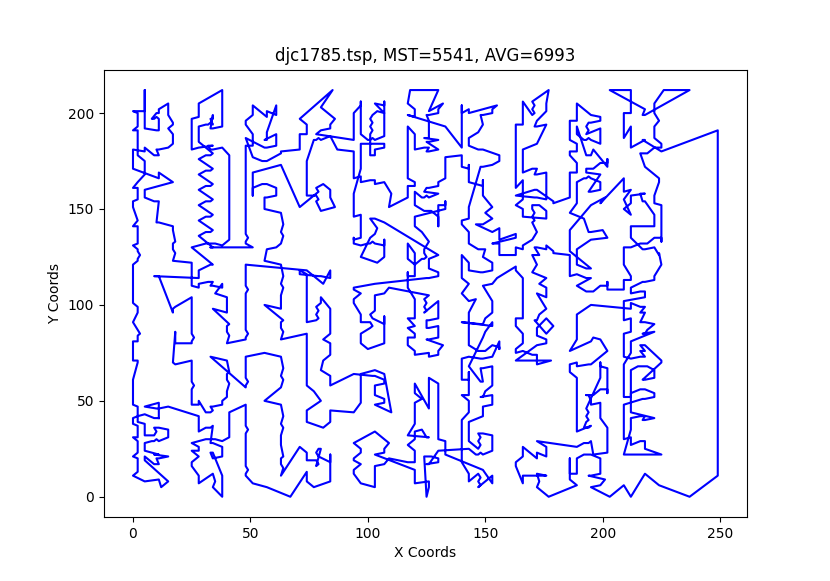
\includegraphics[width=0.8\textwidth, height=10cm]{cycle_1785.png}
\caption{Cykl po Local Searchu dla 100 kroków poprawy}
\label{Newton}
\end{figure}

\begin{figure}[H] 
\centering
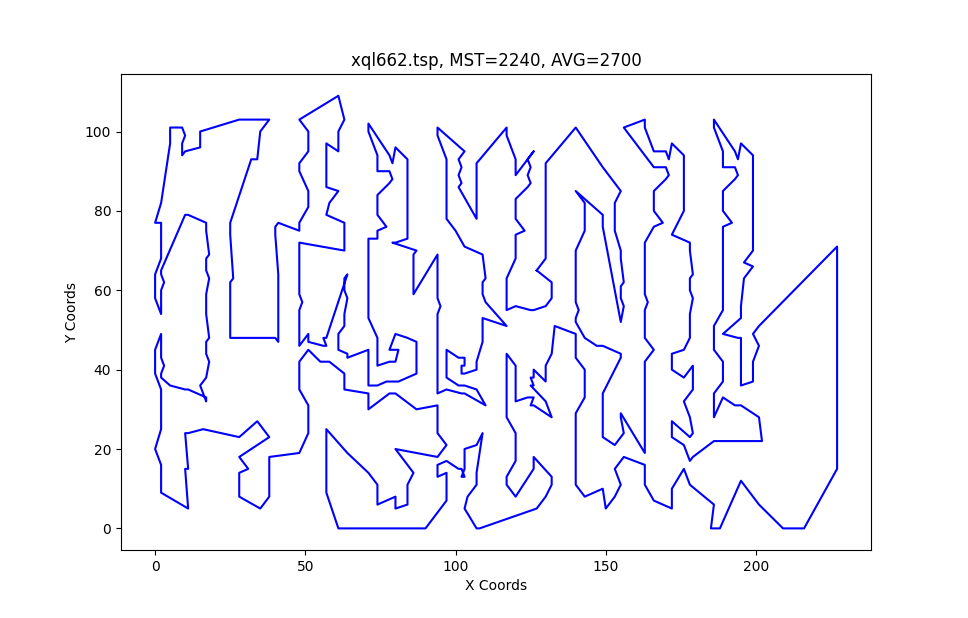
\includegraphics[width=0.8\textwidth, height=10cm]{cycle_662.png}
\caption{Cykl po Local Searchu dla 662 wierzchołków}
\label{Newton}
\end{figure}


\end{document}
